\documentclass[journal]{IEEEtran}

\usepackage{cite,graphicx}
\usepackage[usenames,dvipsnames]{xcolor}

% *** GRAPHICS RELATED PACKAGES ***
%
\ifCLASSINFOpdf
  % \usepackage[pdftex]{graphicx}
  % declare the path(s) where your graphic files are
  % \graphicspath{{../pdf/}{../jpeg/}}
  % and their extensions so you won't have to specify these with
  % every instance of \includegraphics
  % \DeclareGraphicsExtensions{.pdf,.jpeg,.png}
\else
  % or other class option (dvipsone, dvipdf, if not using dvips). graphicx
  % will default to the driver specified in the system graphics.cfg if no
  % driver is specified.
  % \usepackage[dvips]{graphicx}
  % declare the path(s) where your graphic files are
  % \graphicspath{{../eps/}}
  % and their extensions so you won't have to specify these with
  % every instance of \includegraphics
  % \DeclareGraphicsExtensions{.eps}
\fi

\usepackage{graphicx}
\usepackage[cmex10]{amsmath}
\usepackage{algorithmic}
\usepackage{array}
\usepackage{mdwmath}
\usepackage{mdwtab}
\usepackage{eqparbox}
%\usepackage[tight,footnotesize]{subfigure}
%\usepackage[caption=false]{caption}
%\usepackage[font=footnotesize]{subfig}
%\usepackage[caption=false,font=footnotesize]{subfig}
\usepackage{fixltx2e}
\usepackage{stfloats}
\usepackage{url}

% *** Do not adjust lengths that control margins, column widths, etc. ***
% *** Do not use packages that alter fonts (such as pslatex).         ***
% There should be no need to do such things with IEEEtran.cls V1.6 and later.
% (Unless specifically asked to do so by the journal or conference you plan
% to submit to, of course. )

% correct bad hyphenation here
\hyphenation{op-tical net-works semi-conduc-tor}

\begin{document}
%
% paper title
% can use linebreaks \\ within to get better formatting as desired
\title{TODO: A Survey of StarCraft AI Techniques}
%
%
% author names and IEEE memberships
% note positions of commas and nonbreaking spaces ( ~ ) LaTeX will not break
% a structure at a ~ so this keeps an author's name from being broken across
% two lines.
% use \thanks{} to gain access to the first footnote area
% a separate \thanks must be used for each paragraph as LaTeX2e's \thanks
% was not built to handle multiple paragraphs
%

\author{FirstName~LastName,~\IEEEmembership{Member,~IEEE,}
        Jim~Raynor,~\IEEEmembership{Fellow,~RR,}
        and~Sarah~Kerrigan,~\IEEEmembership{Life~Fellow,~ZS}% <-this % stops a space
\thanks{FirstName~LastName is with the Department of Names
GA, 30332 USA e-mail: (see http://www.michaelshell.org/contact.html).}% <-this % stops a space
\thanks{J. Raynor and S. Kerrigane are with the Romeo\&Juliet Inc.}% <-this % stops a space
\thanks{Manuscript received April 19, 2499; revised January 11, 2500.}}

% note the % following the last \IEEEmembership and also \thanks - 
% these prevent an unwanted space from occurring between the last author name
% and the end of the author line. i.e., if you had this:
% 
% \author{....lastname \thanks{...} \thanks{...} }
%                     ^------------^------------^----Do not want these spaces!
%
% a space would be appended to the last name and could cause every name on that
% line to be shifted left slightly. This is one of those "LaTeX things". For
% instance, "\textbf{A} \textbf{B}" will typeset as "A B" not "AB". To get
% "AB" then you have to do: "\textbf{A}\textbf{B}"
% \thanks is no different in this regard, so shield the last } of each \thanks
% that ends a line with a % and do not let a space in before the next \thanks.
% Spaces after \IEEEmembership other than the last one are OK (and needed) as
% you are supposed to have spaces between the names. For what it is worth,
% this is a minor point as most people would not even notice if the said evil
% space somehow managed to creep in.

% The paper headers
\markboth{TCIAIG ~Vol.~X, No.~Y, Month~Year}%
{Shell \MakeLowercase{\textit{et al.}}: TODO: Title here}

\maketitle

\begin{abstract}
TODO: Idea of the paper is: ``one-stop guide on what is the
state of the art in Starcraft AI''. It should help people participating in the competition focus
their efforts, and also should help people implementing AI for RTS games in
general (e.g. industry).  In Gabriel's words ``RTS AI problems, Solutions, State-of-the-art, conclude on what's "solved" since \cite{Buro03rts} and what's not.'' 

For example, if someone wants to implement a bot, and wonders "how should I do scouting", our paper should provide a summary of the existing techniques, and pointers to know more. 
\end{abstract}

\begin{IEEEkeywords}
Game AI, Real-Time Strategy, Starcraft, Review1

\end{IEEEkeywords}

% For peer review papers, you can put extra information on the cover
% page as needed:
% \ifCLASSOPTIONpeerreview
% \begin{center} \bfseries EDICS Category: 3-BBND \end{center}
% \fi
%
% For peerreview papers, this IEEEtran command inserts a page break and
% creates the second title. It will be ignored for other modes.
\IEEEpeerreviewmaketitle

\section{Introduction}\label{sec:intro}
\IEEEPARstart{S}{ince} Michael Buro's call for research in RTS games \cite{Buro03rts}, many researchers have answered the call. Specially, AI competitions like the Starcraft one have caused many AI techniques to be
applied to RTS AI. We will list and classify these approaches, explain their 
power and their downsides and conclude on what is left to achieve human-level 
RTS AI.

{\color{blue}
Motivate the paper, and provide an outline.

Some arguments to use in the motivation could be that games are a good application to motivate novel AI research (as has been happening throughout the history of AI), and that techniques and algorithms developed for RTS games, in addition to be useful and relevant to the game industry, have broader application to other areas.

Reiterate that the goal of this paper is to provide a one-stop guide on what is the
state of the art in Starcraft AI
}

\section{Real-Time Strategy Games}\label{sec:rts}

{\color{blue} [Here, a brief overview of RTS games, which are their main characteristics, etc.]}

\subsection{StarCraft {\color{blue}- Situation}}\label{subsec:starcraft}

Starcraft: Brood War is a popular RTS game released in 1998 by Blizzard Entertainment. Starcraft is set in a science-fiction based world where the player must choose one of the three races: Terran, Protoss or Zerg. The good work done by the people of Blizzard makes this game one of the most extremely well-balanced RTS games ever created.
\begin{itemize}
	\item Terrans, human exiled from Earth, provide units that are versatile and flexible giving a balanced option between Protoss and Zergs.
	\item Protoss units have lengthy and expensive manufacturing process, but they are strong and resistant. These conditions makes players follow a strategy of quality over quantity.
	\item Zergs, the insectoid race, units are cheap and weak. They can be produced fast, encouraging players to overwhelm their opponents with sheer numbers.
\end{itemize}

{\color{blue}TODO: explain the gameplay a little more, how are ppl not familiar to SC able to understand the problems for AI that we raise below?}

\subsection{Challenges in RTS Game AI {\color{blue}- Problems}}\label{subsec:challenges}

{\color{blue}
This section should be brief, and just give us some basic ideas of which are the challenges in RTS Game AI, so that when we refer to related work, we can use this as a reference point.  The most important thing of this section is to demonstrate that RTS games are complex.

Many years have passed since Buro's call for research (8!!). he identified 6 challenges:
\begin{itemize}
\item Resource management
\item Decision making under uncertainty
\item Spatial and temporal reasoning
\item Collaboration
\item Opponent modeling, Learning
\item Adversarial real-time planning
\end{itemize}

There has been a lot of work in many, but others have been untouched (e.g. Collaboration). Additionally, other challenges that are not in the list appeared, and have been worked on, like: how to exploit the existing domain knowledge (strategies, build-orders, replays, etc.), or how to design an architecture that integrates all the modules required for an agent to play an RTS games. 

\begin{itemize}
\item Task Decomposition (or ``Architecture'')
\item Integration of Domain Knowledge
\item Reasoning with Uncertainty (including information gathering)
\item Opponent Modeling and Adaptation: opponent modeling is key if we have to adapt our strategy. As different strategies are dominating each others, forming multiple Nash equilibria, the AI has to be able to infer the intend of its opponent.
\item Group and Individual Control (``micro''): the task of controlling units efficiently (we can not speak of optimality here due to the huge state space, and of the enemy behavior entails numerous Nash equilibria), focusing fire to diminish enemy's firepower and keeping our units alive the longest, casting defensive and offensive spells and abilities.
\item Planning and Resource Allocation (``macro'')
\item Spatial reasoning (``tactics'')
\end{itemize}

Maybe the list above goes better in Section \ref{sec:questions}?
}

{\color{red}
TODO merge above and bottom
}

{\color{blue}
\textbf{Planning}
TODO (Santi?) just a paragraph on exposing why there is a planning problem in RTS AI.

\textbf{Spatial and Temporal Reasoning}
TODO just a paragraph on exposing why there are temporal and spatial reasoning in RTS AI.
}

\textbf{Learning}\\
When talking about learning in RTS games, with regard to a particular match against an opponent (where a match is a sequence of games against the same opponent), one has to differentiate between:
\begin{itemize}
\item Prior learning: done before the match, like when a bot learns what is likely to happen on a given match-up (and map) from replays, or when a bot optimizes its parameters beforehand through simulated annealing or genetic evolution.
\item In-game learning: done between the different actions (decisions) taken during a game. For instance, a bot can take into account the successes and failures of its attacks (location, type, timings).
\item In-match learning: done between the different games of the match, it encompasses opponent modeling across multiple games and adapting the bots' strategy to its successes and failures.
\end{itemize}
Learning in all these situations can be supervised (labeled replays, scripted situations) or unsupervised (unlabeled data, exploratory situations). The last two kinds of situations of learning are more inclined towards reinforcement learning because the AI has to deal with the exploration-exploitation duality. %prior learning: supervised \cite{WeberCIG09} \cite{SynnaeveCIG11}, unsupervised: \cite{SynnaeveAIIDE11}

%%% I think there are two important aspects of uncertainty in RTS games:
%%% \begin{itemize}
%%% \item First is trying to model uncertainty and try to reduce it (information gathering, and representation of knowledge), this includes scouting, and maintaining good estimates of locations and number of units of the enemy, etc.
%%% \item Second is actually using the uncertain information. Taking decisions like army strength estimation (like to attack or retreat).
%%% \end{itemize}

\textbf{Uncertainty}\\
In RTS games, there are two main kinds of uncertainty, existing for two different reasons. First, there is incompleteness of information, due to the fog of war, which leads to some kind of ``extensional'' 
%``extensive'' 
uncertainty, that can be lowered by good scouting, and knowledge representation (to infer what is possible given what has been seen). Secondly, there is the fact that we will never be able to read the opponent's mind, the ``intentional'' 
%or ``intensive'' 
uncertainty that we cannot really be sure to scratch off, even with the best scouting possible. For intentional uncertainty, the AI, as the human player, can only build a sensible model of what the opponent is likely to do, to think, or to think knowing what we think he thinks. Both these kinds of uncertainty can be studied through probabilities, but only for extensional uncertainty can $P(Hidden | Seen)$ be \textit{directly} linked to data. %now for the clumsy part:
One could argue that the extensional data is the only thing that matters because it is the only thing that has an influence on the game, but in reality, for very highly skilled players, discovering the intentions of the enemy is the key to winning. It allows for a compact understanding of the game state and development, while also giving additional information about the future. Whereas a player is doing action A to follow it up by action B or C depends on its intention, while the information about action A is visible and information about B or C is hidden, only intention allows for a choice.



\section{Existing work on RTS Game AI - \color{blue}{Resolutions}}\label{sec:review}

%\subsection{RTS AI Decomposition}
\begin{figure}
    \centering
    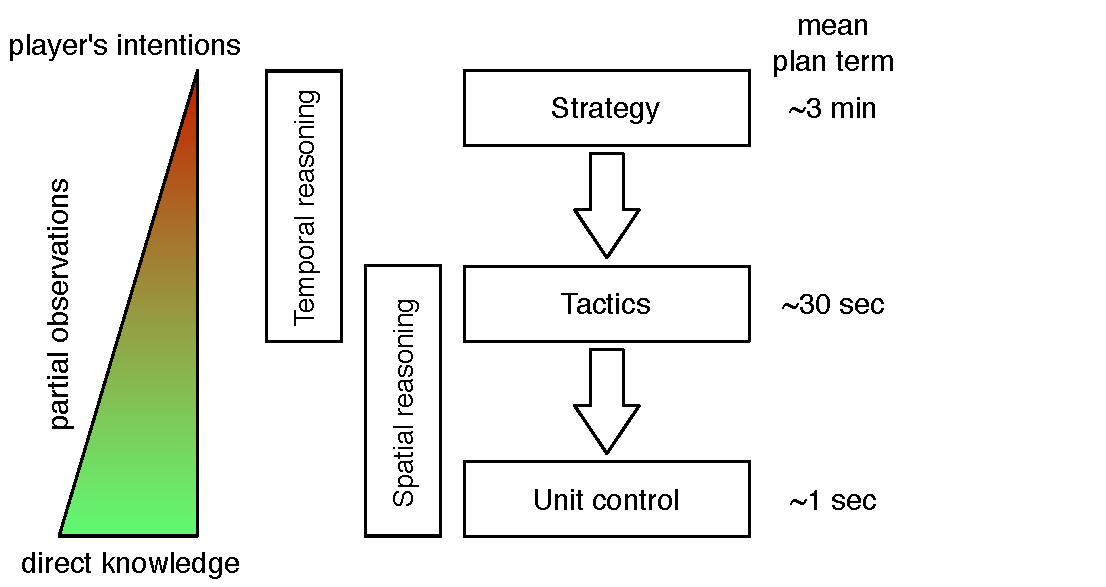
\includegraphics[width=0.9\columnwidth]{figures/levels_abstraction.pdf}
    \caption{RTS AI levels of abstraction and their properties: uncertainty (from intentions and from partial observation) is going higher as the abstraction levels are raising. The timings on the right correspond to an estimate of the duration of a behavior switch in StarCraft. Spatial and temporal reasoning are indicated for part for which greedy solutions are really not efficient.}
    \label{fig:levels-abstraction}
\end{figure}

Systems that play RTS games need to address most, if not all, the aforementioned problems together. Therefore, it is hard to classify existing work on RTS AI as addressing the different problems above. For that reason, in order to classify existing work on RTS AI, we will divide the existing work according to three levels of abstraction (division that is widely used by RTS players): strategy, tactics and reactive control (micro-management). 

Figure~\ref{fig:levels-abstraction} graphically illustrates how strategy, tactics and reactive control are three points in a continuum scale where strategy corresponds to decisions making processes that affect long spans of time (several minutes in the case of Starcraft), reactive control corresponds to low-level second-by-second decisions, and tactics sit in the middle. Also, strategic decisions reason about the whole game at once, whereas tactical or reactive control decisions are localized, and affect only specific groups of units. Typically, strategic decisions constraint future tactical decisions, which in turn condition reactive control. Moreover, information gathered while performing reactive control, can cause reconsideration of the tactics being employed; which could trigger further strategical reasoning.

Following this idea, we consider strategy to be everything related to the technology trees, build-order\footnote{The {\em build-order} is the specific sequence in which buildings of different types will be constructed at the beginning of a game, and completely determines the long-term strategy of a player.}, upgrades, and army composition. It is the most deliberative level, as a player selected and performs a strategy with future stances (aggressive, defensive, economy, technology) and tactics in mind. We consider tactics, everything related to confrontations between groups of units. Tactical reasoning involves both spatial (exploiting the terrain) and temporal (army movements) reasoning, constrained on the possible types of attacks by the army composition of the player and their opponent. Finally, we will call reactive control (also known as micro-management) to how the player controls individual units to maximize their efficiency (when executing tactics) in real-time and adversary conditions. The main difference between tactics and reactive control is that tactical reasoning typically involves some sort of planning ahead for some short spans of time, whereas reactive control involves no planning ahead whatsoever.

% Example:
For example, after starting a game, a player might decide to use a {\em rushing} strategy (which involves quickly building an army and sending it to attack as early as possible in the game); then, when performing the attack use a {\em surrounding} tactic, where the player tries to surround the enemy cutting potential escape routes; finally, while executing the surrounding tactic, the player might decide to use reactive control techniques that command individual units to perform repeated {\em attack and flee} movements, to maximize the efficiency of each of the units being used in the attack.

%{\color{blue}
%perhaps TODO ``how it's done in the industry'' regrouping the first paragraph of each of the following 3 sections?
%}


\subsection{Strategy}
%Every AI needs to observe the world in order to analyze it and take decisions. In RTS games this task isn't trivial since we have to deal with imperfect information.
%The most common decision making are Decision Trees. Some of the advantages of the decision trees are: simple to understand and interpret acting like a white box where we can explain why a decision is taken, and they are compatible with other decision techniques. For complex decisions we have many algorithms to generate an optimum decision tree like ID3 or C4.5, depends on the problem we will use one or another.

% INTRO:
Strategic decision making in real-time domains is still an open problem. In the context of RTS games is has been addressed using many AI techniques, like hard-coded approaches, planning-based approaches, or machine learning-based approaches. Let us cover each of these approaches in turn.

% HARD-CODED:
Hard-coded approaches have been extensively used in commercial RTS games. The most common approaches use finite state machines (FSM) \cite{FSM_AIGameProgWisdom2003} in order to let the AI author hard-code the strategy that the AI will employ. The idea behind FSMs is to decompose the AI behavior into easily manageable states, such as ``attacking'', ``gathering resources'' or ``repairing'' and establish the conditions that trigger transitions between them. Commercial approaches also include Hierarchical FSMs, in which FSMS are composed hierarchically. These hard-coded approaches have achieved a significant amount of success, and, as we will discuss later, have also been used in many academic RTS AI research systems, as discussed in Section \ref{sec:bot}. However, strategic decision making is a hard problem, and these hard-coded approaches struggle to encode dynamic, adaptive behaviors. 

% XXX: Santi: I've commented out this paragraph, since it has nothing to do with RTS games. There is no commercial RTS game using planning (neither STRIPS nor HTN) that I'm aware of. The references below refer to FEAR, which is an FPS game.
%To this end, several approaches have been developed like hierarchical task networks, behavior trees and the comeback of STRIPS \cite{FikesSTRIPS} planning in the industry \cite{orkinGDC_FEAR}. Regardless, one cannot but notice that adaptability is not the strong point of industrial RTS AI. In the context of RTS AI strategy adaptation is related to the idea of opponent modeling. An adapting AI needs to keep track of what the enemy is doing in order to estimate the probability that they will use a specific strategy and adapt its own strategy accordingly. 

% PLANNING:
Approaches using planning techniques have also been explored in the literature. For example Onta\~{n}\'{o}n et al. \cite{CBR_Planning} explored the use of real-time case-based planning (CBP) in the domain of Wargus (a Warcraft II clone). In their work, they used human demonstration to learn plans, that are then composed at run-time in order to form full-fledges strategies to play the game. In \cite{PlanRetrieval} they improve over  their previous CBP approach by using situation assessment for improving the quality and speed of plan retrieval. Hierarchical Task-Network (HTN) planning has also been explored with some success in the context of simpler first-person shooter games. Planning approaches offer more adaptivity of the AI strategy compared to hard-coded approaches. However, the real-time constraints of RTS games limit the planning approaches that can be applied, being HTN and case-based planning the only ones explored so far. Moreover, none of these approaches addresses any timing or scheduling issues, which are key in RTS games.

% MACHINE LEARNING:
Concerning machine learning-based approaches, Weber and Mateas \cite{WeberCig09} proposed ``a data mining approach to strategy prediction'' and performed supervised learning (from buildings features) on labeled StarCraft replays. Dereszynski et al. \cite{HMMstrat_RTS_AIIDE11} used HMM to learn the transition probabilities of sequences of constructions and kept the most probables to produce probabilistic behavior models (in StarCraft). Synnaeve and Bessi\`{e}re \cite{SynnaeveOpeningCig11} used the dataset of \cite{WeberCig09} and presented a Bayesian semi-supervised model to learn from replays and predict openings (early game strategies) from StarCraft replays. The openings are labeled by EM clustering considering appropriate features. Then in \cite{SynnaeveAIIDE11}, they presented an unsupervised learning Bayesian model for tech-tree prediction, still using replays.

% CBR:
Also falling into the machine-learning category, a significant group of researchers has explored case-based reasoning (CBR) \cite{Aamodt94CBR} approaches for strategic decision making. For example Aha et al. \cite{LTW} used CBR to perform dynamic plan retrieval in the Wargus domain. Hsieh and Sun \cite{HsiehS08} based their work on \cite{LTW} CBR model and used StarCraft replays to construct states and building sequences (``build orders''). Finally, Schadd et al. \cite{SchaddBS07} applied a CBR approach to opponent modeling through hierarchically structured models of the opponent behavior and they applied their work to the Spring RTS (Total Annihilation clone).

% SCOUTING:
One final consideration is that RTS games are typically partially observable. For example games like StarCraft implement the ``fog of war'' idea, which basically means that a player can only see the areas of the map close to her own units. Areas of the map away from the field of view of individual units are not observable. Therefore, in order to play an RTS game, players need to scout the opponent in order to obtain information about the opponent's strategy. Very few of the previous approaches deal with this problem, and use perfect information all the time (in the case of commercial games, most AI implementations cheat, since they have perfect information). In commercial games, in order to make the human player believe the built-in AI of this games does scouting, sometimes they simulate some scouting tasks as Bob Fitch described in his AIIDE 2011 keynote for the WarCraft game series and StarCraft: Broodwar. A notable exception is the work of Weber et al. \cite{WeberAIIDE11}, who used a particle model with a linear trajectory update to track opponent units under fog of war in StarCraft. They also produced tactical goals through reactive planning and goal-driven autonomy \cite{WeberCig10,Weber10}, finding the more relevant goal(s) to spawn in unforeseen situations. 

%{\color{ForestGreen}
%Nobody had described an efficient way to scout the opponent... better opponent information better opponent modeling...
%}

\subsection{Tactics}

% INTRO:
Tactical reasoning involves reasoning about the different abilities of the units in a group of units and about the environment (terrain) and positions of the different units in order to gain military advantage in battles. For example, it would be a very bad tactical decision to place fast, invisible or flying units (typically expensive) in the first line of fire against slower heavier units, since they will be wiped out fast. We will divide the work on tactical reasoning in two parts: terrain analysis and decision making.

% TERRAIN ANALYSIS:
Terrain analysis supplies the AI with structured information about the map in order to help making decisions. This analysis is usually performed off-line, in order to save CPU time during the game. For example, Pottinger \cite{Pottinger00} described the \emph{BANG} engine implemented by Ensemble Studios for the game Age of Empires II. This engine provides terrain analysis functionalities to the game using influence maps and areas with connectivity information. 
Forbus et al. \cite{Forbus2002} showed the importance to have qualitative spatial information for wargames, for which they used geometric and pathfinding analysis. 
Hale et al. \cite{Hale08} presented a 2D geometric navigation mesh generation method from expanding convex regions from seeds. 
Finally, Perkins \cite{Perkins10} applied Voronoi decomposition (then pruning) %\cite{Karavelas04}
to detect regions and relevant choke points in RTS maps. This approach is implemented for StarCraft in BWTA\footnote{\url{http://code.google.com/p/bwta/}}.
% Isla 2006 Game AI Programming Wisdom 3. Charles River Media. chapter Probabilistic Target Tracking and Search Using Occupancy Maps, 379–388. ? 

% MACHINE LEARNING:
Concerning tactical decision making, many different approaches have been explored such as machine learning or game tree search. Concerning machine learning approaches, 
Hladky and Bulitko \cite{Hladky2008} benchmarked hidden semi-Markov models (HSMM) and particle filters in first person shooter games (FPS) units tracking. They showed that the accuracy of occupancy maps was improved using movement models (learned from the player behavior) in HSMM. Kabanza et al. \cite{OBRecog} improve the probabilistic hostile agent task tracker (PHATT \cite{PHATT}, a simulated HMM for plan recognition) by encoding strategies as HTN, used for plan and intent recognition to find tactical opportunities. Sharma et al. \cite{CBR-RL} combined CBR and reinforcement learning to enable reuse of tactical plan components. Finally, Cadena and Garrido \cite{CadenaG11} used fuzzy CBR (fuzzy case matching) for strategic and tactical planning. 

% GAME TREE SEARCH:
Game tree search techniques have also been explored for tactical decision making. \cite{Chung05} applied Monte-Carlo planning to a capture-the-flag mod of Open RTS. Balla and Fern \cite{UCT} applied upper confidence bounds on trees (UCT: a MCTS algorithm) to tactical assault planning in Wargus. % (Santi: I commented this one, since it's mentioned above) On influence maps, \cite{teamCompositionRTS} studied team composition and maneuvering by learning a self-organizing map, while \cite{HagelbackJ08} presented a multi-agent potential field based bot.  

% SCOUTING:
Additionally, scouting is equally important in tactical decision making as in strategic decision making. However, as mentioned earlier, very little work has been done in this respect, being that of Weber et al. \cite{WeberAIIDE11} the only exception.


\subsection{Reactive Control}

Reactive control, also called micro-management in RTS games, aims at maximizing the effectiveness of units, including simultaneous control of units of different types in complex battles on heterogeneous terrain. 

% POTENTIAL FIELDS:
Potential fields (or influence maps) have been found to be a useful technique for reactive decision making. Some uses of potential fields in RTS games are: avoiding obstacles (navigation), avoiding opponent fire, or staying at maximum shooting distance \cite{Hagelback08,Hagelback09}. Hagelb\"{a}ck and Johansson \cite{HagelbackJ08} presented a multi-agent potential fields based bot able to deal with fog of war in the Tankbattle game. Avery et al. \cite{Avery09} and Smith et al. \cite{SmithCIG10} co-evolved influence map trees for spatial reasoning in RTS games. Danielsiek et al. \cite{Danielsiek_2008} used influence maps to achieve intelligent squad movement to flank the opponent in a RTS game. A drawback for potential field-based techniques is the large number of parameters that has to be tuned in order to achieve the desired behavior. Approaches for automatically learning such parameters have been explored, for example, using reinforcement Learning \cite{Liu_2008}, or self-organizing-maps (SOM) \cite{teamCompositionRTS}. We would like to note that potential fields are a reactive control technique, and as such, they do not perform any form of lookahead. As a consequence, these techniques are prone to make units stuck in local optima. 


% Machine learning:
There has been a significant amount of work on using machine learning techniques for the problem of reactive control. Bayesian modeling has been applied to inverse fusion of the sensory inputs of the units \cite{SynnaeveMicroCig11}, which subsumes potential fields, allowing for integration of tactical goals directly in micro-management. 
Additionally, there has been some interesting uses of reinforcement learning (RL) \cite{Sutton}: Marthi et al. \cite{Marthi05} employ concurrent hierarchical Q-learning (units Q-functions are combined at the group level) RL to efficiently control units in a ``one robot with multiple effectors'' fashion. Madeira et al. \cite{Madeira06} advocate the use of prior domain knowledge to allow faster RL learning and applied their work on a turn-based strategy game. In real game setups, the actions spaces to explore is gigantic, it requires to use the structure of the game in a partial program (or a partial Markov decision process) and a shape function (or a heuristic) \cite{Marthi05}. Other approaches that aim at learning the parameters of an underlying model have also been explored. For example Ponsen and Spronck \cite{GA} used evolutionary learning techniques, but face the same problem of dimensionality. The difficulty to work with multi-scale goals and plans is handled directly by case-based reasoning (CBR), which has been adapted for units behavior with continuous action models \cite{Molineaux08}, an integrated RL/CBR algorithm using continuous models, or with hybrid CBR/RL transfer learning \cite{CBR-RL}. Reactive planning \cite{WeberCig10}, a decompositional planning similar to hierarchical task networks \cite{HTNPlanning}, allows for plans to be changed at different granularity levels and so for multi-scale (hierarchical) goals integration of low-level control. Synnaeve and Bessi\`{e}re \cite{SynnaeveMicroCig11} achieve hierarchical goals (coming from tactical decisions) integration through the addition of another sensory input corresponding to the goal's objective.

% Other:
Other research falling into reactive control has been performed in the field of cognitive science, where Wintermute et al. \cite{SORTS} have explored human-like attention models (with units grouping and vision of a unique screen location) for micro-management.

% Pathfinding:
Finally, although pathfinding does not fall under our previous definition of reactive control, we include it in this section, since it is typically performed as a low-level service, not part of either tactical nor strategical reasoning (although there are some exceptions, like the tactical pathfinding of Danielsiek et al. \cite{Danielsiek_2008}). The most common pathfinding algorithm is A*, but its big problem is CPU time and memory consumption, hard to satisfy in a complex, dynamic, real-time environment with large numbers of units. Even if specialized algorithms, such as D*-Lite \cite{KoenigL02} exist, it is most common to use A* combined with a map simplification technique that generates a simpler navigation graph to be used for pathfinding. An example of such technique is Triangulation Reduction A*, that computes polygonal triangulations on a grid-based map \cite{Demyen_2006}. Considering movement for groups of units, rather then individual units, techniques such as steering of flocking behaviors \cite{Reynolds_1999} can be used on top of a path-finding algorithm in order to make whole groups of units follow a given path. In recent commercial RTS games like Starcraft 2 or Supreme Commander 2, flocking-like behaviors are inspired of continuum crowds (``flow field'') \cite{Treuille2006}. A comprehensive review about (grid-based) pathfinding was recently done by Sturtevant \cite{sturtevant2012benchmarks}.

\subsection{Holistic Approaches}

{\color{red} [Santi: some RTS AI techniques attempt to address the problem in a holistic way, for example the Darmok system, is there enough work on this for justifying a whole subsection? or should we just spread the few pieces of work on this over the previous sections].}

\section{State of the Art Bots for Starcraft - \color{blue}{Information/Productions}}\label{sec:bot}

Thanks to the recent organization of international game AI competitions focused around the popular StarCraft game (see Section \ref{sec:competition}), several groups have been working on integrating many of the techniques described in the previous section into complete ``bots'', capable of playing complete StarCraft games. In this section we will overview some of the currently available top bots, and focus, first on the architecture being used to integrate all the techniques being used for the different aspects of the bot, and then on which subsets of techniques are used for each bot.

\subsection{RTS Bot Architectures}\label{sec:integration}

Playing an RTS game involves dealing with all the problems described above. A few approaches, like CAT \cite{LTW}, Darmok \cite{OntanonMSR10} or ALisp \cite{Marthi05} try to deal with the problem in a monolithic manner, by using a single AI technique. This resembles approaches to solve other games, such as Chess or Go, where a single game-tree search approach is enough to play the game at human level. However, none of those systems aims at achieving near human performance. In order to achieve human-level performance, RTS AI designers use a lot of domain knowledge in order to divide the task of playing the game into a collection of sub-problems, which can be dealt-with using individual AI techniques (as discussed in the previous section). 

\begin{figure*}[ta]
    \centering
    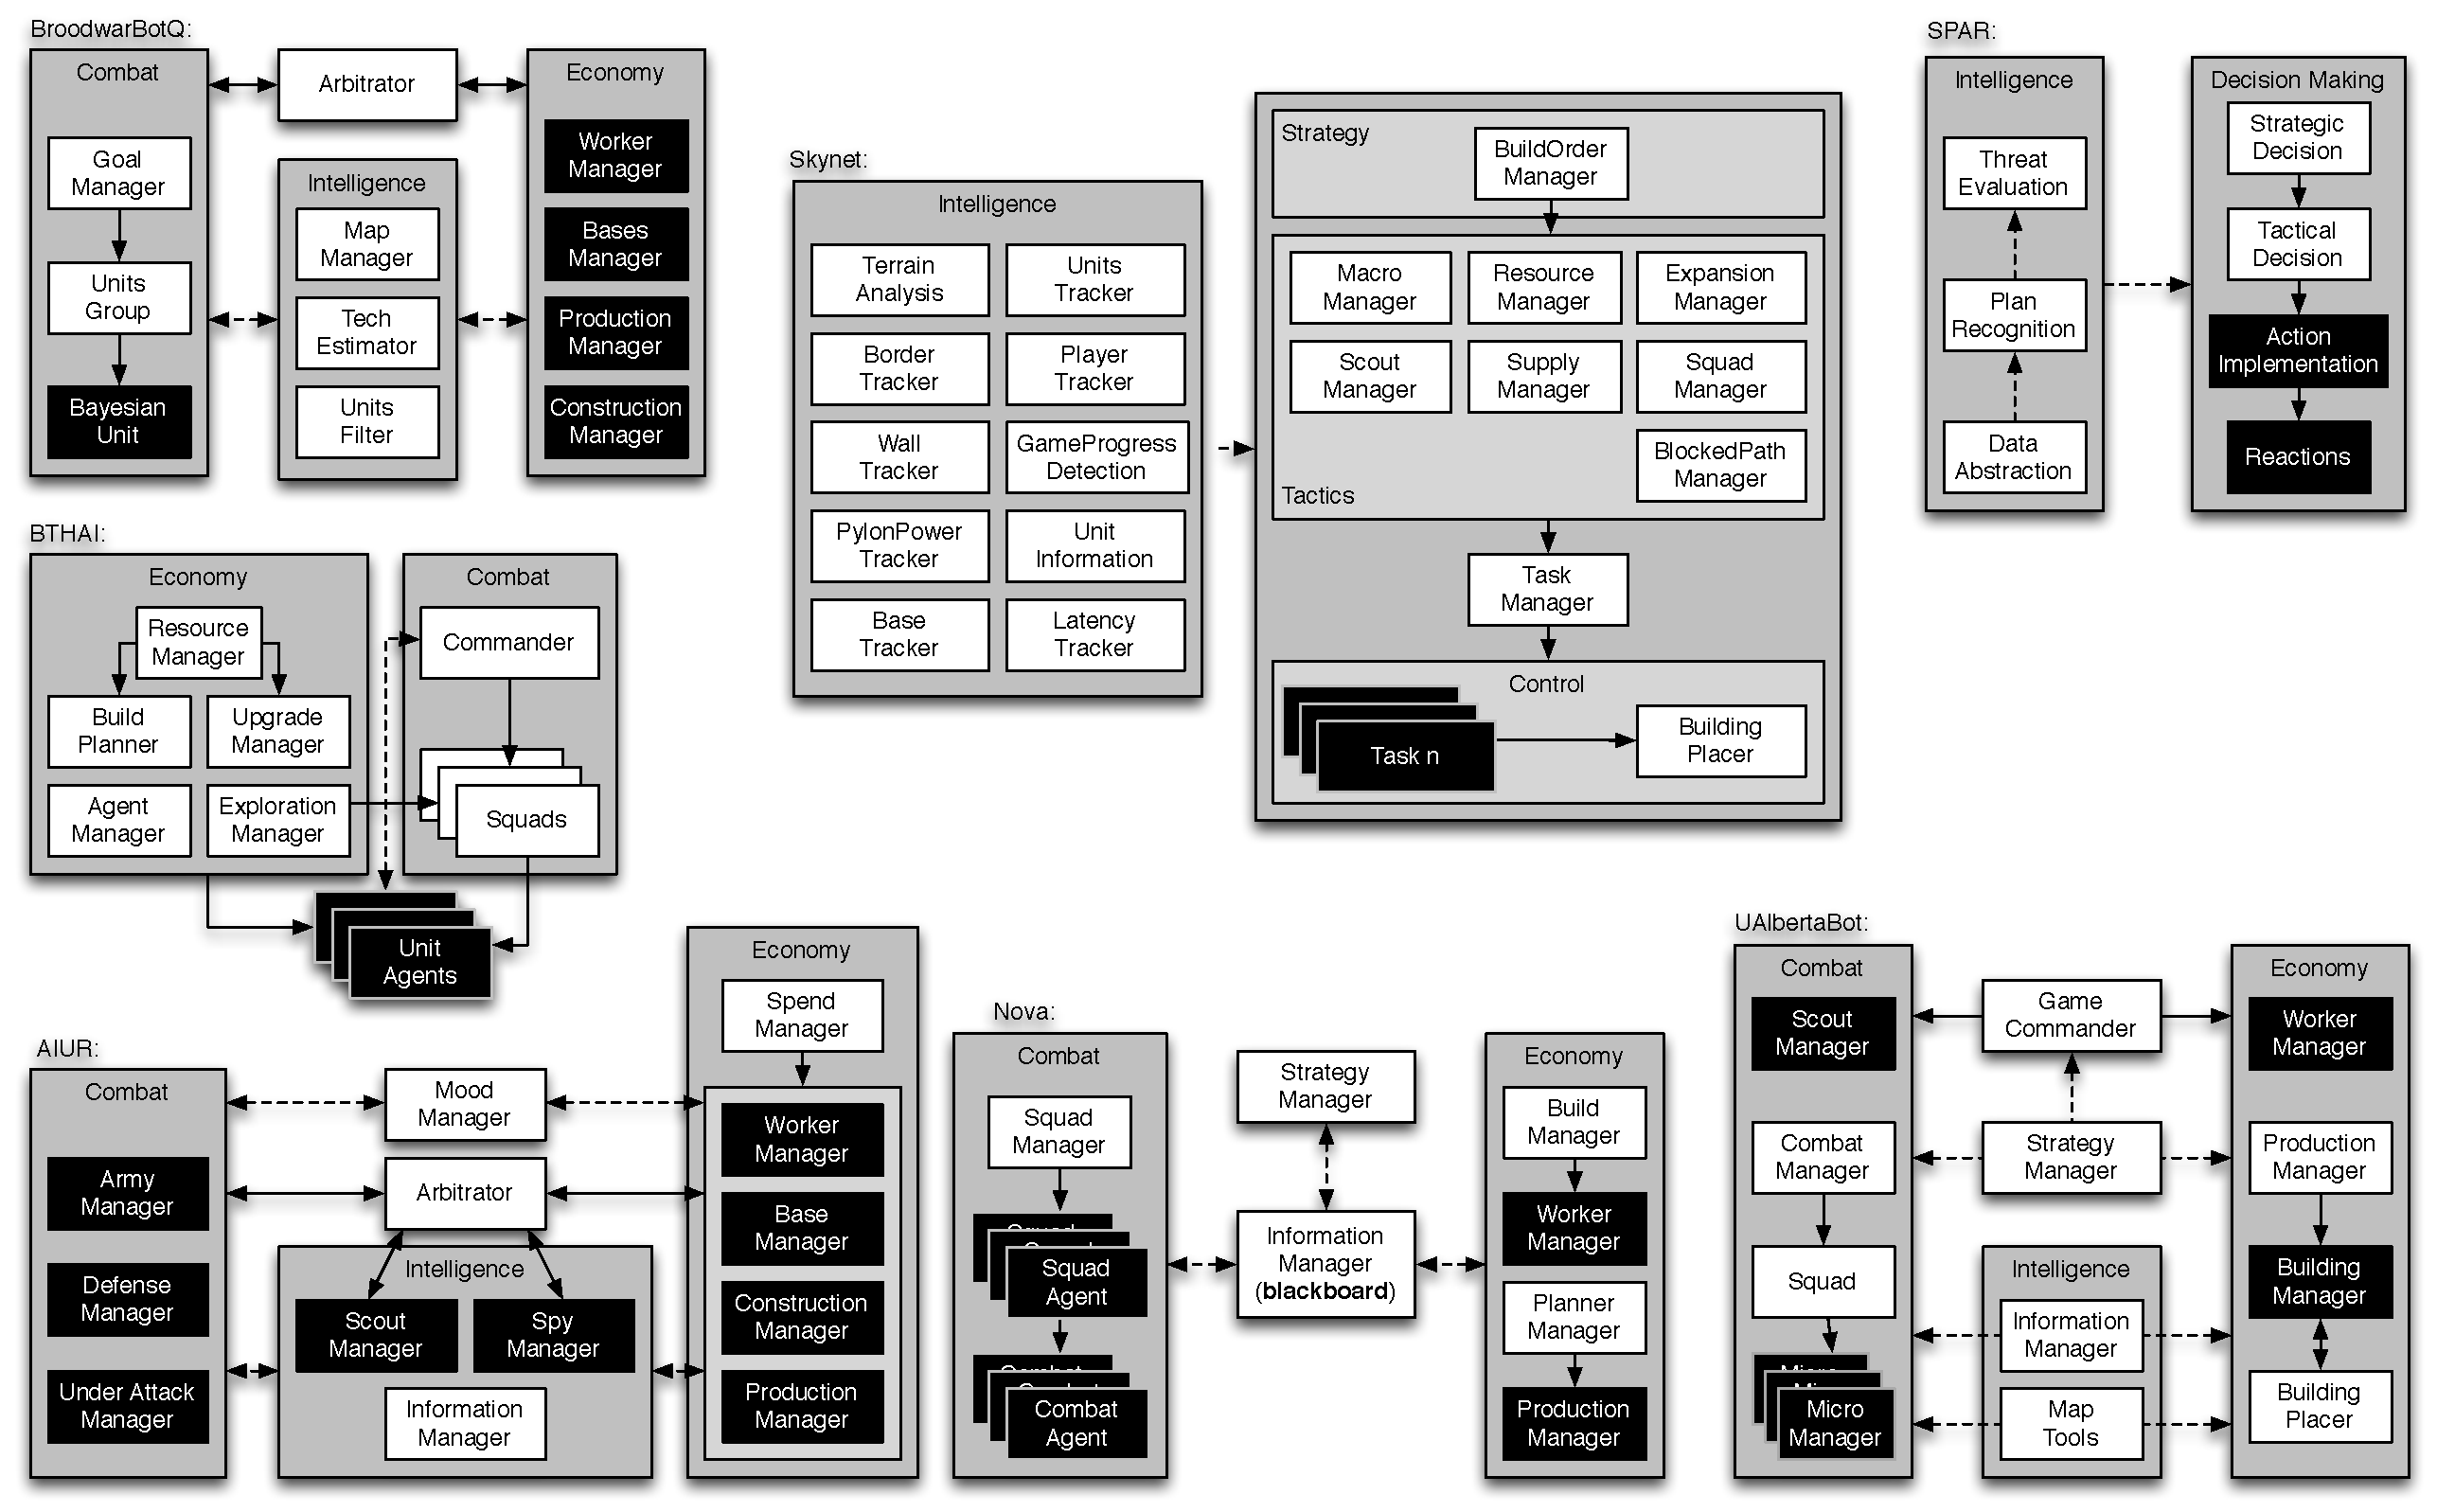
\includegraphics[width=\textwidth]{figures/figure-bot-architectures-wide.pdf}
    \caption{Architecture of 6 Starcraft bots obtained by analyzing their source code. Modules with black background sent commands directly to Starcraft, dashed arrows represent data flow, and solid arrows represent control.}
    \label{fig:bot-architecture}
\end{figure*}

Figure \ref{fig:bot-architecture} shows some representative examples of the integration architectures used by different bots in the AIIDE and CIG 2011 Starcraft AI competitions \cite{url1,url2}: BroodwarQ \cite{???}, Nova \cite{???}, UAlbertaBot \cite{???}, Skynet \cite{???}, SPAR \cite{???}, AIUR \cite{???}, and BTHAI \cite{???} (see Section \ref{sec:competition} for a comparison of their performance). Each box represents an individual module with a clearly defined task (only modules with a black background can send actions directly to Starcraft). Dashed arrows represent data flow, and solid arrows represent control (when a module can command another module to perform some task). For example, we can see how SPAR is divided in two sets of modules: {\em situation analysis} and {\em decision making}, the first with three modules dedicated to analyze the current situation of the game, and the later with 4 modules dedicated to exploit that information to decide what to do. We can see how the decision making aspect of SPAR is organized hierarchically, with the higher-level module ({\em strategic decision}) issuing commands to the next module ({\em tactical decision}), which sends commands to the next module ({\em action implementation}), and so on. Only the lower-level modules can send actions directly to Starcraft. 

On the other hand, bots such as NOVA or BroodwarBotQ (BBQ) only use a hierarchical organization for {\em micro-management} (controlling the attack units), but use a decentralized organization for the rest of the bot. In Nova and BBQ, there is a collection of modules that control different aspects of the game (workers, production, construction, etc.). These modules can all send actions directly to Starcraft. In Nova those modules coordinate mostly through writing data in a shared blackboard, and in BBQ they coordinate only when they have to use a shared resource (unit) by means of an arbitrator.

By analyzing the structure of these bots, we can see that there are two main tools that can be used when designing an integration architecture:

\begin{itemize}
\item {\em Abstraction}: complex tasks can be formulated at different levels of abstraction. For example, playing an RTS game can be seen as issuing individual low-level actions to each of the units in the game, or at a higher level, it can be seen as deploying a specific strategy (e.g. a ``BBS strategy'', or a ``Reaver Drop'' strategy). Some bots, reason at multiple levels of abstraction at the same time, making the task of playing Starcraft simpler. Assuming that each module in the architecture of a bot has a goal and determines some actions to achieve that goal, the actions determined by higher-level modules are considered as the goals of the lower level modules. In this way, each module can focus on reasoning at only one level of abstraction, thus, making the problem easier.

\item {\em Divide-and-conquer}: playing a complex RTS, such as Starcraft, requires performing many conceptually different tasks, such as gathering resources, attacking, placing buildings, etc. Assuming each of these tasks can be performed relatively independently and without interference, we can have one module focusing on each of the tasks independently, thus making the problem easier. 
\end{itemize}

If we imagine the different tasks to perform in a complex RTS game in a two-dimensional plane, where the vertical axis represents abstraction, and the horizontal axis represents the different aspects of the game (micro-management, resource gathering, etc.), abstraction can be seen as dividing the space with horizontal lines, whereas divide-and-conquer divides the space using vertical lines.

Different bots, use different combinations of these two tools. Looking back at Figure \ref{fig:bot-architecture}, we can see the following use of abstraction and divide-in-conquer in the bots:

\begin{itemize}
\item BroodwarBotQ: uses abstraction for micro-management, and divide-and-conquer for macro-management and intelligence gathering. To avoid conflicts between modules (since the individual tasks of each of the modules are not completely independent), BBQ uses an arbitrator.
\item Nova: is similar in design as BroodwarBotQ, and uses abstraction for micro-management, and divide-and-conquer for macro-management. The differences are that Nova does not have an arbitrator to resolve conflicts, but has a higher-level module ({\em strategy manager}), which posts information to the blackboard that the rest of modules follow (thus, making use of abstraction).
\item UAlbertaBot: also uses abstraction in micro-management like the previous two bots. But it also uses it in macro-management: as can be seen, the production manager sends commands to the building manager, who is in charge of producing the buildings. This bot also uses divide-and-conquer, and tasks like scouting and resource gathering are managed by separate, independent modules.
\item Skynet: makes extensive use of both abstraction and divide-and-conquer. Considering the decision making component of Skynet, we can see a high level module that issues commands to a series of tactics modules. The collection of tactic modules queue {\em tasks} (that are analogous to the abstract actions used in SPAR). Each different task has a specific low level module that knows how to execute it. Thus, Skynet uses a 3 layered abstraction hierarchy, and uses divide-and-conquer in all levels except the highest.
\item SPAR: only uses abstraction. Its high-level module determines the strategy to use, and the tactical decision module divides it into a collection of {\em abstract actions}, that are executed by the lower-level modules.
\item AIUR: is mainly divide-and-conquer oriented, for macro as well as for micro, with a slight abstraction on macro with a SpendManager deciding how to spend resources among Base, Production and Construction Managers. At the beginning of a game, the MoodManager initializes a ``mood'' which will influence both micro and macro. For example, micro-management is divided into three independent managers: the {\em Defense Manager}, controlling military units when there is nothing special, the {\em Under Attack Manager}, activated when the opponent is attacking our bases, and the {\em Army Manager}, taking control of units when it is time to attack, following a timing given by the current mood.
\item BTHAI: uses a two-tier abstraction hierarchy, where a collection of high-level modules command a collection of lower-level agents in charge of each of the units. At the high-level, BTHAI uses divide-and-conquer, having multiple high-level modules issuing commands to the lower-level units.
\end{itemize}

Additionally, except for BTHAI, all other agents use divide-and-conquer at a higher-level bot design and divide all the modules into two or three categories: {\em information gathering} and {\em decision}, or {\em information gathering}, {\em micro-management} and {\em macro-management}.

Some bots using divide-and-conquer, assume that each of the modules can act independently and that their actions can be executed without interference. BBQ, UAlbertaBot and AIUR, however use an arbitrator ({\em Game Commander'} in UAlbertaBot) that makes sure that modules do not send contradictory orders to the same unit. However, very little bots handle the problem of how to coordinate resource usage amongst modules, for instance BTHAI uses a first-come-first-serve policy for spending resources, the first module that requests resources is the one that gets them. Nova and Skynet are exceptions, and implement some rudimentary prioritization based on the high level strategy. Following available resources and timing, AIUR's {\em Spend Manager} orders Base, Production and Construction Managers what they have to build/produce. It also orders to start tech research and upgrades.

One interesting aspect of the five bots described above is that, while all of them are reactive at the lower level (reactive control), most if not all of them, are scripted at the highest level of abstraction. BTHAI reads build and squad formations from a predefined script, Nova's {\em Strategy Manager} is a predefined finite-state machine, BBQ's construction manager reads the build order from a predefined script, and Skynet's {\em BuildOrder Manager} is basically a predefined script. Such scripts describe the strategy that the bots will use, however, such strategy is always fixed. One could see this pre-scripting as if each bot defined a ``high-level programming language'' to describe Starcraft strategies, and the bots themselves are just interpreters of such strategy. Compared to current approaches for Chess or Go, this scripting seems a rigid and inflexible, but responds to the much higher complexity of the Starcraft game. An interesting exception to that is UAlbertaBot, which uses a search algorithm in the {\em Production Manager} to find near-optimal build orders. Another interesting case is AIUR, that uses a {\em Mood Manager} to randomly pick a mood among five (rush, aggressive, defensive, macro, fast expand), which will influence the build order, strategy and tactics, all of them scripted so far. This mood can change during the game, following the opponent behavior.

In conclusion, we can see that there are two basic tools that can be used in an integration architecture: abstraction and divide-and-conquer, which are widely used by the existing Starcraft bots. 

This section has focused on discussing the architecture of existing Starcraft bots. Let us now focus on what is the state of the art on the techniques used for each of the individual modules used by them.

\subsection{Individual AI Techniques}\label{sec:techniques}

{\color{red} TODO}

\section{Recent Starcraft AI Competitions}\label{sec:competition}

{\color{violet}

In order to inject new AI code into the StarCraft game, all recent
tournaments attached to scientific conferences employ the 
Brood War Application Programming Interface 
(BWAPI)\footnote{\url{http://code.google.com/p/bwapi/}} which 
enables replacing the human player interface with a C++ library,
some auxiliary libraries and the bot code. A consequence of this
indirect way of integrating new bots is that every machine can
only run one custom bot, requiring two computers for a 2-player game.

\subsection{AIIDE}
\label{sec:AIIDE}
this is left empty for now


\subsection{CIG 2011}
\label{sec:cig2011}

An initial attempt to run a StarCraft tournament at the Computational
Intelligence in Games conference 2010 suffered from technical problems.
These mainly stemmed from the desire to use evolved, largely untested
maps which proved to look interesting but made the submitted bots 
(and/or the Broodwar Terrain Analyzer (BWTA) provided with the BWapi interface) crash
so frequently that it would have been unjustifiable to announce a winner.

At CIG 2011, the tournament was therefore run with a (secret) selection
of maps used in league play, which can be regarded as the most important
difference to the AIIDE tournament that employed a known list of maps.
The competition was organized by Tobias Mahlmann and Mike
Preuss and attracted 10 bots. In addition to the ones discussed in previous
sections (UAlbertaBot, Skynet, AIUR, Nova, BroodwarBotQ, BTHAI), 
the set also contained LSAI, Xelnaga, Protoss Beast Jelly, and EvoBot,
these are shortly described in the following:

\paragraph*{LSAI (Zerg)} utilizes a heavily modified BWSAL to divide management
 of the units to different modules that communicate via a centralized information
 module. It works using a simple reactive strategy to try and survive early game
 attacks and macro up to a larger attack force and maintain map control.
 
\paragraph*{Xelnaga (Protoss)} is a modification of the AIUR bot that chooses the 
Dark Templar Opening in order to destroy the enemy base before defenses against
invisible units are available. 

\paragraph*{Protoss Beast Jelly (Protoss)}
always goes for a 5-gate Zealot rush, supported by an effective harvesting 
strategy named power-mining (2 probes are assigned to every mineral patch,
thereby needing 18 probes for 100\% saturation in a normal map, prior
to expanding). Gas is not mined as it is not needed for constructing Zealots.

\paragraph*{EvoBot (Terran)} employs an evolutionary algorithm for obtaining rational
 unit combinations and influence map techniques for deciding the strategic locations. Note
 that this bot was submitted in a very early version, with many of its designed features not
 yet fully ready. 


\begin{table*}[htb]
\caption{Results of the first round at CIG 2011, held in two brackets.
Qualified for the final round: UAlbertaBot and Skynet (from A), Xelnaga
and BroodwarBotQ (from B, the latter by comparing direct encounters
with BTHAI of which 6:4 were won).}
\label{tab:cig-first-round}
\begin{small}
\begin{center}
% bracket A
\begin{tabular}{|l|c|c|c|}
\hline
\multicolumn{4}{|c|}{Bracket A} \\ \hline
Crashes & games & bot	& wins\\ \hline
0 &	 40 &	 UAlbertaBot &	 33\\
1 &   40 &	 Skynet	  &  31\\
2 &	 40 &	 AIUR	  &  24\\
1 &	 40 &	 Nova	  &  8\\
0 &	 40 &	 LSAI	  &  4\\
\hline
\end{tabular}
% bracket B
\begin{tabular}{|l|c|c|c|}
\hline
\multicolumn{4}{|c|}{Bracket B} \\ \hline
Crashes & games & bot	& wins\\ \hline
12 &	 40 &	 Xelnaga &	 25\\
3 &   40 &	 BroodwarBotQ  &  23 (6)\\
0 &	 40 &	 BTHAI	  &  23 (4)\\
17 &	 40 &	 Protoss Beast Jelly  & 17\\
0 &	 40 &	 EvoBot	  &  12\\
\hline
\end{tabular}
\end{center}
\end{small}
\end{table*}

\subsubsection{First Round}
\label{sec:cig-first-round}

As the CIG competition games were executed manually due to
a lack of available software (the AIIDE program was not yet
available at that time), we separated the ten entries into
two brackets. In each bracket of 5 bots, a round-robin
tournament was held with 10 repetitions per pairing, resulting
in 40 games per bot.
The 5 maps chosen for the first round were selected from the pool
of well-known league play maps found on the internet:
\emph{(2)MatchPoint 1.3}, \emph{(4)Fighting Spirit 1.3}, 
\emph{iCCupdestination 1.1}, \emph{iCCup gaia}, and 
\emph{iCCup great barrier reef}. Each bot pairing played
on every map twice, with switched starting positions.

The two top bots of every bracket qualified
for the final round. Table~\ref{tab:cig-first-round} summarizes
the results.
Note that as BroodwarBotQ and BTHAI have the same number of wins,
their direct encounter was evaluated which accounted 6:4 for the BroodwarBotQ.
The bots going into the final were thus UAlbertaBot, Skynet (from bracket A)
and Xelnaga and BroodwarBotQ (from bracket B). All qualified bots play the
Protoss faction. Most bots proved pretty stable, only Xelnaga and Protoss 
Beast Jelly crashed relatively often (each in more than a quarter of the games). 
Crashing of course resulted in an instant win for the other bot.
In some cases, neither bot was able to finish the other off completely,
so that they went into a passive state. We manually ended such games after
around 15 minutes and assigned victory to the bot that had obtained more
points as indicated on the end game screen.


\subsubsection{Final Round}
\label{sec:cig-final-round}

The final round was played in a similar mode as each of the
first round brackets,
using another set of 5 previously unknown maps:
\emph{iCCup lost temple 2.4}, \emph{iCCup rush hour 3.1},
\emph{iCCup swordinthemoon 2.1}, \emph{iCCup yellow 1.1},
and \emph{La\_Mancha 1.1}. 
Letting each pairing play on each map twice again with
switching starting positions resulted in 30 games per bot.
The final results are displayed in table~\ref{tab:cig-final-round},
indicating Skynet as winner and UAlbertaBot as runner-up, being
almost equally strong, and the two other bots as clearly inferior.


\begin{table}[bth]
\caption{Results of the CIG 2011 final round.}
\label{tab:cig-final-round}
\begin{small}
\begin{center}
% bracket A
\begin{tabular}{|l|c|c|c|}
\hline
Crashes & games & bot	& wins\\ \hline
0 &  30 &	 Skynet	  		&  26\\
0 &	 30 &	 UAlbertaBot 	&  22\\
3 &	 30 &	 Xelnaga  		&  11\\
2 &	 30 &	 BroodwarBotQ  	&  1\\
\hline
\end{tabular}
\end{center}
\end{small}
\end{table}


}



\section{Open Questions in RTS Game AI}\label{sec:questions}

{\color{blue}
[This is a preliminary list of open questions, derived from the Skype call on July 19. Some work is still required to turn this into the final list]
}

As illustrated in this paper, there is a set of problems in RTS game AI that could be considered mostly solved, of for which we have very good solutions. One example of such problems is pathfinding (mostly solved) or micro-management (we have good solutions). 

However, there are many other problems for which this is not the case. For example, there is no current Starcraft bot that can come up with its own tactical moves, such as ``unit drops''. Some bots do drops, but only if this is hard-coded; no bot has the capability of reasoning about the current situation, synthesize a tactical move that involves a ``unit drop'', and determine that this move is the best one in the current situation. This is related to the lack of real-time adversarial planning techniques that scale up to the size required for RTS games. Similarly, current bots do not exhibit adaptation to opponent strategies. Some switch between different build-orders, but do not fully adapt their strategy. No bot is capable of observing the opponent and autonomously synthesize a good plan from scratch to counter the opponent strategy.

Specifically, the list of problems that are currently unsolved, grouped in various categories:

{\color{blue}

\begin{itemize}

\item Learning and adaptation:
\begin{itemize}
\item Adaptation to opponent strategy.
\item Learning from experience in RTS games.
\item Learning from observation (from demonstration, or from observing the opponent) in RTS games.
\end{itemize}

\item Planning:
\begin{itemize}
\item Adversarial planning under real-time constraints (there is some work on this area to be presented this year in AIIDE).
\item Adversarial planning under uncertainty.
\item Adversarial planning in partially-observable domains.
\item Adversarial planning with resources (there exist planning algorithms that handle resources, like GRT-R, but cannot scale up to the size of problems needed for e.g. Starcraft).
\end{itemize}

\item Scalability:
\begin{itemize}
\item How to scale up existing algorithms for adversarial domains like game tree search or Monte Carlo search to the very large dimensions of RTS games.
\end{itemize}

\item Integration:
\begin{itemize}
\item Multi-scale planning/reasoning: how to integrate reasoning at multiple levels of abstraction.
\end{itemize}

\item Domain Knowledge: 
\begin{itemize}
\item we know how to incorporate some aspects of domain knowledge (e.g. build orders), but, in general, how to incorporate some forms of domain knowledge into algorithms for RTS games is still an open problem. For example, standard techniques to encode strategies for other forms of games, like Behavior Trees, are hard to deploy in RTS games. 
\end{itemize}
\end{itemize}
}


\section{Empirical Evidence of What is Missing in Existing Bots}\label{sec:experiments}

{\color{blue}
Here, whatever experiments we want to include to support which aspects of RTS Game AI require more work.
}

\section{Discussion and Conclusions}\label{sec:conclusions}



\section*{Acknowledgments} {\color{blue} This research is partially funded by projects ... and ... . The authors would like to thank Florian Richoux, author of the AIUR bot, for his helpful comments and help in early drafts of this paper. }



% Can use something like this to put references on a page
% by themselves when using endfloat and the captionsoff option.
\ifCLASSOPTIONcaptionsoff
  \newpage
\fi

%\begin{thebibliography}{1}
%\end{thebibliography}
\bibliographystyle{IEEEtran}                                                    
\bibliography{survey}

%\begin{IEEEbiographynophoto}{FirstName LastName}
%Biography text here.
%\end{IEEEbiographynophoto}

\begin{IEEEbiography}[{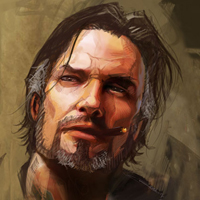
\includegraphics[width=2cm, keepaspectratio]{jim.jpg}}]{Jim Raynor}
Jim Raynor was a Confederate marshal on Mar Sara at the time of the first zerg incursions on that world. He is now with Raynor's Raiders Inc.
\end{IEEEbiography}

\end{document}


In his AIIDE 2010 keynote, Chris Jurnet described the technique XXX, implemented by [COMPANY] in the game YYY \cite{gameurl}
